\section{Semantik}


\exewidth{\exnrfont(124)}


\author{Stefan Müller}


\frame{
\frametitle{Semantik: Material}


\citew{Zimmermann2001a-u}


}

\author{Stefan Müller (Ede Zimmermann)}

\subsection{Wörtliche Bedeutung}

\frame{
\frametitlefit{Wörtliche Bedeutung -- Verborgener Sinn, Ironie, Implikatur}


\begin{itemize}
\item Den Untersuchungsgegenstand der Semantik bilden sprachliche Inhalte bzw.\ \blaubf{Sinn} und
  \blaubf{Bedeutung} (Wir unterscheiden terminologisch nicht zwischen Sinn und Bedeutung).
\pause
\item Nicht alles, was man mit einer Äußerung assoziiert, gehört zur Semantik.
\begin{itemize}
\item Verborgener Sinn (Gedichte)
\pause
\item Ironie und Implikatur
\eal
\ex Das Steak war wie immer zart und saftig.\\(je nach Mensa ironisch)
\ex Der Nachtisch war nicht giftig.\\(Implikatur je nach Kontext $\to$ schlecht)
\zl
\end{itemize}
\end{itemize}

}

\frame{
\frametitle{Wörtliche Bedeutung -- Stil, Metaphern}

\begin{itemize}
\item Nicht alles, was man mit einer Äußerung assoziiert, gehört zur Semantik.
\begin{itemize}
\item Wortwahl und Stil kann Sprechereinstellungen übermitteln:
\eal
\ex Willst Du allen Ernstes für den Fraß noch mehr Kohle verlangen?
\ex Planen Sie tatsächlich eine Anhebung der Essenspreise?
\zl
(duzen, \emph{Fraß}, \emph{wollen} unhöflich, \emph{allen Ernstes} abwegig?, \emph{Kohle} Slang)

\pause
\item Sprachliche Bilder:
\eal
\ex Fußballer = Terrier (Laufstil, Aussehen, Charakter)
\ex Klagelied meines Kühlschranks
\zl

Geräusch der Kühlschranks klingt wie Klagelied $\to$ Vergleich\\
(\mex{0}b) ist dagegen eine Metapher, da offen bleibt,\\
worin der Vergleich besteht.

\end{itemize}
\end{itemize}

}

\frame{
\frametitle{Metaphern}

\begin{itemize}
\item Metaphern können verblassen und eine wörtliche Bedeutung annehmen:
\ea
fadenscheinig
\z
Zusätzlich zur alten Bedeutung (Qualität eines Gewebes) gibt es eine neue: Qualität der
Selbstrechtfertigung.

\pause
Man sagt, die Metapher ist \blaubf{erstarrt}.

\pause
\item Was ist der wörtliche Sinn von (\mex{1})?
\ea
Die Ausflüchte des Terriers waren fadenscheinig.
\z
Nur \emph{Terrier} ist metaphorisch verwendet, \emph{fadenscheinig} ist in wörtlicher Lesart
verwendet worden:
\ea
Ein Hund hat schlechte Ausreden vorgebracht.
\z


\end{itemize}

}

\begin{frame}
\frametitle{Metapher oder nicht?}
  \begin{itemize}
  \item Wann ist eine Metapher erstarrt? Das kann man nicht genau festlegen, da die Übergänge
    fließend sind.
\pause
\item Trotzdem ist eine scharfe Trennung für bestimmte Zwecke sinnvoll: semantische Theoriebildung.
\pause
\item Abgrenzung erlaubt getrennte Bearbeitung der Bereiche,\\ mit verschiedenen Methoden.
\pause
\item Semantik beschäftigt sich mit der wörtlichen Bedeutung und alles was über den reinen Wortsinn
  hinausgeht ist Gegenstand der Pragmatik.
  \end{itemize}
\end{frame}

\subsection{Lexikalische Semantik}

\begin{frame}
\frametitle{Lexikalische Semantik}

  \begin{itemize}
  \item Die Bedeutung eines komplexen Ausdrucks ergibt sich aus der Bedeutung seiner Teile + der
    Art, wie diese kombiniert wurden.

\pause

\item Das nennt man \blaubf{Frege-Prinzip}, obwohl Frege es selbst in seinen Texten nicht explizit
  formuliert hat.

\pause
  \item Frage: Was bedeuten die Teile?
  \end{itemize}
\end{frame}

\begin{frame}
\frametitle{Homonymie und grammatische Eigenschaften}

\begin{itemize}
  \item Es ist möglich, dass ein "`Wort"' mehrere Lesarten hat.

Man spricht dann von \blaubf{Homonymie}: 
\eal
\ex der/die Kiefer -- die Kiefer/die Kiefern
\pause
\ex der/das Bauer -- die Bauern/die Bauer
\pause
\ex \visible<4->{das} {Band} \pause\visible<4->{({Bänder}) -- der {Band} ({Bände}) -- die {Band} ({Bands})}
\zl

Die Wörter unterscheiden sich im Genus.

  \end{itemize}
\end{frame}




\frame{
\frametitle{Homonymie: Plural}

\begin{columns}[T]

\begin{column}{45mm}
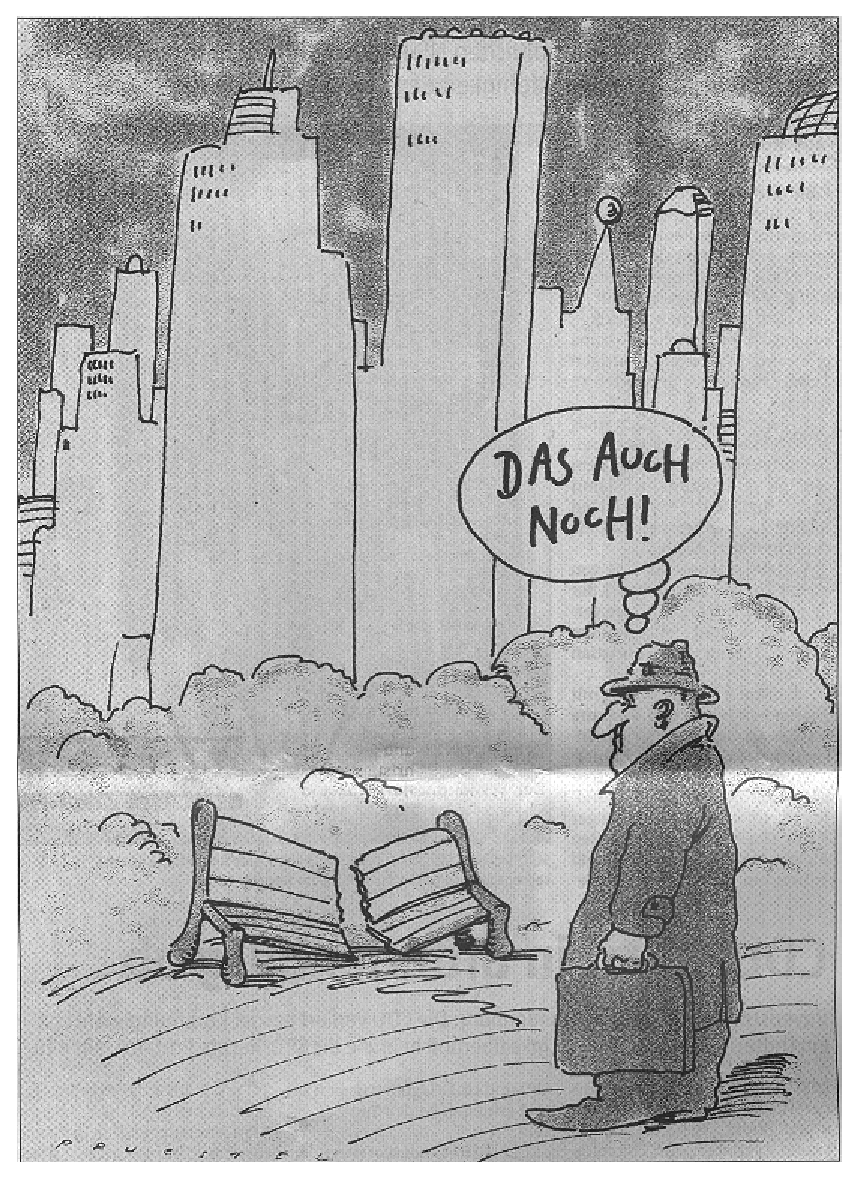
\includegraphics[width=\textwidth]{Bilder/bankenkrise}
\end{column}
\begin{column}{73mm}
Genusunterschiede nicht immer gegeben:
\eal
\ex die Bank -- die Banken
\ex die Bank -- die Bänke
\zl
\end{column}
\end{columns}
}

\frame{
\frametitle{Homonymie: grammatisch unmarkiert}



\includegraphics[width=0.6\textwidth]{Bilder/300px-Ostteil_Sanssouci}\hfill
\includegraphics[width=0.3\textwidth]{Bilder/180px-Burgwaechter_Schloss_mit_Schluessel}

Wieviele Schlösser sind hier zu sehen?

}


\begin{frame}
\frametitle{Homophone und Homographen}
  \begin{itemize}
  \item \blaubf{Homophone}
\eal
\ex Miene (Gesichtsausdruck) 
\ex Mine (Bergwerk, Sprengkörper, Stift) 
\zl
\pause
\item \blaubf{Homographen} 
\eal 
\ex übers\textprimstress etzen 
\ex \textprimstress übersetzen
\zl
\pause
\item Solche Identität von Formen ist aber relativ uninteressant,\\
      weil zufällig oder historisch begründet.
  \end{itemize}
\end{frame}


\begin{frame}
\frametitle{Polyseme}
  \begin{itemize}
  \item Interessanter sind Polyseme:
\eal
\ex Krone: Königskrone, Baumkrone, Schaumkrone
\ex belegen: ein Seminar/einen Platz/eine Aussage/ein Brötchen belegen
\zl
Die Lesarten unterscheiden sich, sind aber miteinander verwandt.

\pause
\item Produktive Polysemien interessant, weil sich dafür Regeln finden lassen.

Beispiel: \blaubf{Metonymie}: gemeinter Gegenstand wird durch einen Ausdruck bezeichnet, der sich
auf einen anderen, aber verbundenen Gegenstand bezieht. \zb Teil für Ganzes.
\ea
Möchtest Du noch eine Tasse? = \\Möchtest Du noch eine Tasse gefüllt mit Tee?
\z
Genauso \emph{Glas}, \emph{Teller}: Gefäß für Inhalt

  \end{itemize}
\end{frame}

\begin{frame}
\frametitle{Polysemie}
  \begin{itemize}
  \item Tier für sein Fleisch.
\eal
\ex Dort drüben läuft ein Kaninchen. 
\ex Zu Ostern gab es Kaninchen.
\zl
  \end{itemize}
\end{frame}

\author{Stefan Müller}


\subsection{Bedeutung von Ausdrücken}

\begin{frame}
\frametitle{Bedeutung von Ausdrücken: \emph{Kind}}

Ein Nomen bezieht sich auf eine Menge von Objekten,\\
        die die entsprechenden Eigenschaft haben:\\
        \emph{Kind} steht für alle Kinder in einer bestimmten Situation.

%\centerline{%
\begin{pspicture}[unit=8mm](-1,0)(11,4.5)
%\psgrid
\rnode{D}{\psframe(0,0)(8,5)}
\pscircle[fillcolor=beamer@fugreen,fillstyle=solid](1,1){0.1}
\pscircle[fillcolor=beamer@fugreen,fillstyle=solid](2,2){0.1}
\pscircle[fillcolor=beamer@fugreen,fillstyle=solid](4,2){0.1}
\pscircle[fillcolor=beamer@fugreen,fillstyle=solid](3,3){0.1}
\pscircle[fillcolor=beamer@fugreen,fillstyle=solid](7,4){0.1}
\rput[Bl](5,3){%
\rnode{Kind}{Kind}}
%
\cnode(3,2){1.5}{KindSet}
\ncline[nodesepA=0pt,nodesepB=2pt]{KindSet}{Kind}
%
\rput[Bl](9,2){%
\rnode{Diskursuniversum}{\begin{tabular}{@{}l@{}}
                         Diskurs-\\
                         universum (Welt)\\
                         \end{tabular}}}
%\ncline[nodesepA=0pt,nodesepB=2pt]{D}{Diskursuniversum}
\psline(8.9,2.4)(8,2.4)
%
%
%\psellipse(4,2)(3,1.5)
%\anodeconnect[l]{modell}[r]{phen}%
\end{pspicture}
%}


\end{frame}


\begin{frame}
\frametitle{Bedeutung von Ausdrücken: Eigennamen}

Eigennamen bezeichnen Individuen.\\
Ein Individuum kann mehrere Namen haben oder keinen.

%\centerline{%
%{
\begin{pspicture}[unit=8mm](-1,0)(11,4.5)
%\psgrid
\psframe(0,0)(8,5)
\rput[Bl](2.6,1.2){%
\rnode{Max}{Max}}
\rput[Bl](1,3){%
\rnode{Dicker}{Dicker}}
\rput[Bl](4,3){%
\rnode{Chantalle}{Chantalle}}
\rput[Bl](2,.5){%
\rnode{Barbara}{Barbara}}

\cnode[fillcolor=beamer@fugreen,fillstyle=solid](1,1){0.1}{BarbaraDot}
\cnode[fillcolor=beamer@fugreen,fillstyle=solid](2,2){0.1}{MaxDot}
\cnode[fillcolor=beamer@fugreen,fillstyle=solid](4,2){0.1}{NonameDot}
\cnode[fillcolor=beamer@fugreen,fillstyle=solid](3,3){0.1}{ChantalleDot}
\cnode[fillcolor=beamer@fugreen,fillstyle=solid](7,4){0.1}{NoName2Dot}
%
%\psellipse(4,2)(3,1.5)
%\anodeconnect[l]{modell}[r]{phen}%
\ncline[nodesepA=2pt,nodesepB=0pt]{Barbara}{BarbaraDot}
\ncline[nodesepA=2pt,nodesepB=0pt]{Max}{MaxDot}
\ncline[nodesepA=2pt,nodesepB=0pt]{Dicker}{MaxDot}
\ncline[nodesepA=2pt,nodesepB=0pt]{Chantalle}{ChantalleDot}
\end{pspicture}
%}


\end{frame}


\begin{frame}
\frametitle{Bedeutung von Ausdrücken: \emph{klug}}

        \emph{klug} steht für alle klugen Individuen in einer bestimmten Situation.

%\centerline{%
%{
\begin{pspicture}[unit=8mm](-1,0)(11,4.5)
%\psgrid
\psframe(0,0)(8,5)
\pscircle[fillcolor=beamer@fugreen,fillstyle=solid](1,1){0.1}
\pscircle[fillcolor=beamer@fugreen,fillstyle=solid](2,2){0.1}
\pscircle[fillcolor=beamer@fugreen,fillstyle=solid](4,2){0.1}
\pscircle[fillcolor=beamer@fugreen,fillstyle=solid](3,3){0.1}
\pscircle[fillcolor=beamer@fugreen,fillstyle=solid](7,4){0.1}
\rput[Bl](3,0.5){%
\rnode{klug}{klug}}
%
\cnode(1.5,1.5){1}{klugSet}
\ncline[nodesepA=0pt,nodesepB=2pt]{klugSet}{klug}
\end{pspicture}
%}


\end{frame}



\begin{frame}
\frametitle{Bedeutung von Ausdrücken: \emph{kluges Kind}}

Ein \emph{kluges Kind} ist sowohl klug als auch Kind.

%\centerline{%
%{
\begin{pspicture}[unit=8mm](-1,0)(11,4.5)
%\psgrid
\psframe(0,0)(8,5)
\rput[Bl](5,3){%
\rnode{Kind}{Kind}}
%
\cnode(3,2){1.5}{KindSet}
\ncline[nodesepA=0pt,nodesepB=2pt]{KindSet}{Kind}
\rput[Bl](0.5,3.5){%
\rnode{klug}{klug}}
%
\cnode(1.5,1.5){1}{klugSet}
\ncline[nodesepA=0pt,nodesepB=2pt]{klugSet}{klug}
\psclip
{%
\pscircle(3,2){1.5}
}
\pscircle[fillstyle=hlines](1.5,1.5){1}
\endpsclip
\pscircle[fillcolor=beamer@fugreen,fillstyle=solid](1,1){0.1}
\pscircle[fillcolor=beamer@fugreen,fillstyle=solid](2,2){0.1}
\pscircle[fillcolor=beamer@fugreen,fillstyle=solid](4,2){0.1}
\pscircle[fillcolor=beamer@fugreen,fillstyle=solid](3,3){0.1}
\pscircle[fillcolor=beamer@fugreen,fillstyle=solid](7,4){0.1}
%
%\psellipse(4,2)(3,1.5)
%\anodeconnect[l]{modell}[r]{phen}%
\end{pspicture}
%}


\end{frame}


\begin{frame}
\frametitle{Bedeutung von Ausdrücken: \emph{Alle klugen Kinder schlafen}}

\emph{Alle klugen Kinder schlafen} ist in folgender Welt wahr:

%\centerline{%
%{
\begin{pspicture}[unit=8mm](-1,0)(11,4.5)
%\psgrid
\psframe(0,0)(8,5)
\rput[Bl](5,3){%
\rnode{Kind}{Kind}}
%
\cnode(3,2){1.5}{KindSet}
\ncline[nodesepA=0pt,nodesepB=2pt]{KindSet}{Kind}
\rput[Bl](0.5,3.5){%
\rnode{klug}{klug}}
%
\cnode(1.5,1.5){1}{klugSet}
\ncline[nodesepA=0pt,nodesepB=2pt]{klugSet}{klug}
\psclip
{%
\pscircle(3,2){1.5}
}
\pscircle[fillstyle=hlines](1.5,1.5){1}
\endpsclip
\pscircle[fillcolor=beamer@fugreen,fillstyle=solid](1,1){0.1}
\pscircle[fillcolor=beamer@fugreen,fillstyle=solid](2,2){0.1}
\pscircle[fillcolor=beamer@fugreen,fillstyle=solid](4,2){0.1}
\pscircle[fillcolor=beamer@fugreen,fillstyle=solid](3,3){0.1}
\pscircle[fillcolor=beamer@fugreen,fillstyle=solid](7,4){0.1}
%
\rput*[refpoint]{45}(2.5,-1){\psellipse(2.5,2.5)(1.8,0.9)}
\rput[Bl](4.5,4){%
\rnode{schlafen}{schlafen}}
\psline(4.3,4.1)(3.8,3.8)
\ncline[nodesepA=0pt,nodesepB=2pt]{schlafenSet}{schlafen}
%\anodeconnect[l]{modell}[r]{phen}%
\end{pspicture}
%}

Für alle, für die gilt, dass sie klug und Kinder sind, gilt auch,\\
dass sie schlafen. 

\end{frame}

\begin{frame}[shrink=15]
\frametitle{Bedeutung von Determinatoren}

Determinatoren: \zb Quantoren (ein, alle), definite Artikel 
\eal
\ex Alle Kinder schlafen.
\ex Für alle x, für die gilt, dass sie Kind sind, gilt auch, dass sie schlafen.
\ex \blau{$\forall$}x kind(x) \blau{$\to$} schlafen(x)
\zl
\pause
\eal
\ex Ein Kind schläft.
\ex Es gibt mindestens ein Kind und für dieses Kind gilt, dass es schläft.
\ex \blau{$\exists$}x kind(x) \blau{$\wedge$} schlafen(x)
\zl
\pause
\eal
\ex Das Kind schläft.
\ex Es gibt ein (bestimmtes) Kind und für dieses Kind gilt, dass es schläft.
\ex \blau{\textiota}x kind(x) \blau{$\wedge$} schlafen(x)
\zl


\end{frame}

\begin{frame}
\frametitle{Die Bedeutung von Sätzen}

\begin{itemize}
\item Einen Satz verstehen, heißt wissen, was der Fall ist, wenn er wahr ist. (Wittgenstein)
\pause
\item Ein Satz charakterisiert eine Menge von Situationen (mögliche Welten).

\pause

\bigskip

\item Wenn Sie wissen wollen, wie man von den Wörtern zur Gesamtbedeutung kommt, besuchen Sie die Veranstaltung zur Logik/Satzsemantik.

\end{itemize}

\end{frame}

\subsection{Bedeutungsbeziehungen}

\frame{
\frametitle{Semantische Relationen zwischen Wörtern}

\begin{itemize}[<+->]
\item    Synonymie 

        \begin{tabular}[t]{@{}l@{~--~}l}
        {\em Orange}        & {\em Apfelsine}\\
        {\em Telefon}       & {\em Fernsprecher}\\
        {\em Stockwerk\/}   & {\em Etage\/}\\
        {\em Ostzone\/}     & {\em DDR\/}\\
        {\em Morgenstern\/} & {\em Abendstern\/} = Venus\\
        \end{tabular}
\item    Antonymie 

        \begin{tabular}[t]{@{}l@{~--~}l}
        {\em heiß}  & {\em kalt}\\
        {\em Höhen} & {\em Tiefen}\\
        \end{tabular}
\item   Hyperonymie (Oberkonzept),  Hyponymie (Unterkonzept)

        \begin{tabular}[t]{@{}l@{~--~}l}
        {\em Früchte}  & {\em Äpfel}\\
        {\em arbeiten} & {\em schuften}\\
        \end{tabular}
\end{itemize}

}

\frame{
\frametitle{Semantische Relationen zwischen Sätzen}

\begin{itemize}[<+->]
\item Äquivalenz 

        {\em Peter ist kein Papagei.} -- {\em Es ist nicht wahr, dass Peter ein Papagei ist.}

        {\em Wir wählten Klaus.} -- {\em Klaus wurde von uns gewählt.}

\item Kontradiktion 

        {\em Peter ist kein Papagei.} -- {\em Peter ist ein Papagei.}

        {\em Kein Baby kann sprechen.} -- {\em Es gibt einen sprechenden Säugling.}

\item Folgerung, Enthaltensein 


        {\em Sowohl Karl als auch Richard hat Email.} -- {\em Karl hat Email.}

        {\em Das Glas war rot.} -- {\em Das Glas war farbig.}
\end{itemize}
}
